\chapter{Base Station Implementation and Usage}\label{app:rtk_gps}
This appendix contains a description how the RTK GPS base station is implemented and how to use it.

\section*{RTK GPS Basics}
The inaccuracies of GPS receivers are mostly due to atmospheric changes, which add a verity of disturbances dependent on the weather, temperature etc.
The most significant error to be corrected is the ambiguity resolution. Ambiguity resolution is a fixed offset that the GPS receiver experiences as the number of wavelengths from the satellite to the receiver is unknown. This results in a integer which needs to be resolved to improve the accuracy of the GPS measurements. If the ambiguity resolution is not found, the gained precision from other sources is mostly irrelevant due to the bias. \cite{novatel} \cite{RTK_GPS} \cite{ambg_res}

Most modern GPS receivers have a precision of 2-5 m. For applications where this precision is insufficient, an RTK GPS can be used. By comparing the measurements received from a base station, the rover is able to compensate for these disturbances. The base station is a stationary GPS receiver with a known position, which streams correction data, to be used by the rover. The increased precision gained from including a base station is done by assuming the position errors are correlated. As long as the rover remains within a close distance to the base station, this is a good assumption. The rover uses the correction data received form the base to estimate errors. This results in the position being improved by orders of magnitude. 
%The increased performance is a result of the weather pattern is locally similar, meaning that if the base station and the rover is close (within 10-20 km) to each other, the disturbances they experience is the same.
The further the rover gets from the base, the more the noises start to become uncorrelated, resulting in a loss in accuracy. \cite{EmlidRTK} \cite{RTK_GPS}
%This enables the rover to compensate for the weather patterns, granted the base station received the same satellites as the rover.




%%http://www.novatel.com/an-introduction-to-gnss/chapter-5-resolving-errors/real-time-kinematic-rtk/
%%https://www.e-education.psu.edu/geog862/node/1828
%%http://www.wasoft.de/e/iagwg451/intro/introduction.html
%The inaccuracies of GPS receivers is mostly due to atmospheric changes, which adds a verity of disturbances dependent on the weather, temperature etc.
%This results in most modern GPS receivers having a precision of 2-5 m. 
%For applications where this precision is insufficient, an RTK GPS can be used. 
%By comparing the measurements received from a base station, the rover is able to compensate for the disturbances.
%The base station is a stationary GPS receiver with a known position, which streams correction data, to be used by the rover. 
%The increased performance is a result of the weather pattern is locally similar, meaning that if the base station and the rover is close (within 10-20 km) to each other, the disturbances they experience is the same.
%As long as the rover remains within a close distance to the base station, the rover will be able to use the offset the base station experiences to improve it's own measurements.
%This enables the rover to compensate for the weather patterns, granted the base station received the same satellites as the rover.
%This can result in down to sub centimeter precision for some high grade implementations.

\section*{Base Station Implementation and Usage}
The correction data is used by the rover to estimate signal disturbances, caused be the signals entering the atmosphere. 
This enables it to increase the precision of its GPS measurements. This data is formatted as a RTCM3 message, which is a protocol designed for this purpose.
\begin{figure}[H]
	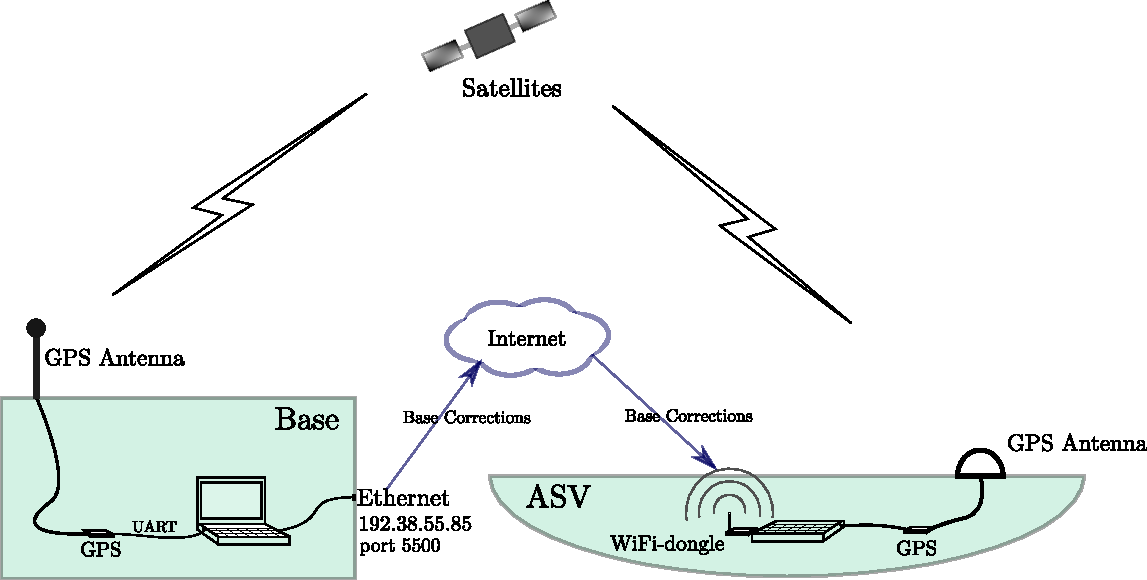
\includegraphics[width=0.6\textwidth]{figures/comunicationSetup.pdf}
	\caption{Overall setup of the GPS.}
	\label{fig:app_gps_setup}
\end{figure}
\autoref{fig:app_gps_setup} shows how the RTK gps system is setup. 
The computer forwards the message to a TCP socket, making it accessible through the Internet. 
%%%%appendix%%%%%%%%%%%%
The Reach is able to act both as a base station and as a rover depending on the settings.
The settings pane is accessed by typing the IP of the module in a browser, which connects to a GUI server hosted by the module after initialization.
In order to get the best possible measurements, the base is set to "static mode" in "RTK settings".
%The emlid reach is setup to send the RTCM3 messages through a USB interface to a computer, acting as a bridge between the university servers and the outside. This setting is found under the "base mode" pane in the GUI.
The computer runs a server capable of reading the serial data, and forwards in the correct package sizes.

The correction data from the base station consists of different message types, varying in length.

Each message contains header, data and a checksum. The header contains information on message type and packet size, which is used to forward the right amount of bytes each time.
Through testing, it has been found that the header is initiated with a hex value of d3, indicating that a new package begins. As the data is transmitted binary, this pattern is not a guarantee that a message is transmitted. 
To ensure the correct package sizes is sent, an initialization sequence is ran on the server at startup, which searches for the initialization sequence, finds the packet size, then reads that amount of bytes, until a package is received with that length, followed by another start sequence.
This can be validated using the checksum, however this feature is yet to be implemented. 

The package size is obtained by locating the initialization sequence to find the header containing the package size. The base station is implemented to cast the RTCM3 message on a TCP socket on IP: 192.38.55.85 Port: 5500. Users with access to the Internet are able to access this socket from anywhere. Under the "Correction Input" pane, the method of input can be selected, if the module has Internet connection, these can be acquired by selecting the "TCP" and client mode, and typing in the IP and Port Number in their respective fields.

The Reach RTK is setup using the ReachView app, which is accessed as a html page, hosted by the reach itself. 
Throughout this project ReachView v. 2.3 is used.
Under the RTK settings page following changes have been applied:
	\begin{itemize}
		\item Ambiguity Resolution (AR) mode is set to Fix and Hold
		\item GNSS selection is: GPS+Glonass+SBAS+QZSS
		\item SNR mask: 15
		\item Elevation Mask Angle: 15
	\end{itemize}
Under Correction input, the following settings are used: 
	\begin{itemize}
		\item TCP is selected for input
		\item Role is Client
		\item IP: 192.38.55.85
		\item PORT: 9000
	\end{itemize}
These settings are only viable in cases where the Emlid Reach has access to the Internet.
This will connect the rover to the base station, such that the correction data is received. 
In cases where it is not possible for the Reach to access the Internet directly, the GPS node is able to forward the correction input through USB. 
In this case following settings are used: 
	\begin{itemize}
		\item USB-To-PC is selected for input
		\item Baud Rate: 115200
	\end{itemize}

%Through this the rover is setup to fix and hold the integer ambiguity, which theoretically improves the stability of the measurements. 



